\item A small body $A$ starts sliding from the height $h$ down an inclined groove passing into a half-circle of radius $h/2$ (Fig. 1.31).
    \begin{center}
        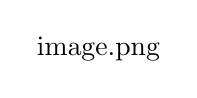
\begin{tikzpicture}
            \node at (0, 0) {{image.png}};
        \end{tikzpicture}
    \end{center}
    Assuming the friction to be negligible, find the velocity of the body at the highest point of its trajectory (after breaking off the groove).
\begin{solution}
    \begin{center}
        \begin{tikzpicture}
            \pic at (0, 0) {frame=3cm};
        \end{tikzpicture}
    \end{center}
    
    \begin{align*}
        \intertext{To complete a smooth vertical track of radius $R$, the minimum height at which a particle starts, must be equal to $\frac{5}{2}R$. Let us first prove this.}
        \intertext{In the figure there is a smooth track and a small body is released at height $h$. We have to find minimum value for $h$ so that the body can complete smooth vertical track of radius $R$. As the track is smooth and the body is under the action of only two forces, normal reaction and gravitational pull. The mechanical energy of the block in the gravitational field is conversed, because normal reaction does zero work whereas the gravitational force is conservative. From the conservation of mechanical energy between the point of release and the upper most point of the circular track}
        \Delta T + \Delta U_{gr} &= 0\\
        \left(\dfrac{1}{2}mv^2 - 0\right) - mg\left(b - 2R\right) &= 0\\
        v^2 &= 2g\left(b - 2R\right)\tag{1}
        \intertext{which yields}
        \intertext{To complete the vertical circular track the condition is that the normal reaction at the upper most point of the circular track $N \geq 0$.}
        \intertext{From Newtons second law in projection form towards the centre of the track}
        F_n &= mw_n \quad (\text{where } w_n \text{ is the normal acceleration})\\
        N + mg &= m\dfrac{v^2}{R}\\
        N &= m\left(\dfrac{v^2}{R} - g\right)
        \intertext{As $N \geq 0$ at upper most point of the circular track}
        m\left(\dfrac{v^2}{R} - g\right) &\geq 0\\
        \intertext{or}
        v^2 &\geq gR\tag{2}
        \intertext{From Eqs. (1) and (2)}
        2g\left(b-2R\right) &\geq gR\\
        b &\geq \dfrac{5}{2}R
        \intertext{Thus in our problem, the body could not reach the upper most point of the vertical track of radius $R/2$. Let the particle $A$ leave the track at some point with speed $v$ (see figure). Now from energy conservation for the body $A$ in the field of gravity}
        mg\left[b-\dfrac{b}{2}(1+\sin\theta)\right] &= \dfrac{1}{2}mv^2\\
        \intertext{or}
        v^2 &= gb(1-\sin\theta)\tag{3}
        \intertext{At the break off point the normal reaction $N=0$, so from Newton's second law at this point}
        F_n &= mw_n\\
        mg\sin\theta &= \dfrac{mv^2}{(b/2)}
        \intertext{So,}
        v^2 &= \dfrac{gb}{2}\sin\theta\tag{4}
        \intertext{From Eqs. (3) and (4),}
        \sin\theta &= \dfrac{2}{3} \quad \text{and} \quad v = \sqrt{\dfrac{gb}{3}}
        \intertext{After leaving the track, the body $A$ comes in air and further goes up and at maximum height of its trajectory in air and its velocity (say $v'$) becomes horizontal. Hence, the sought velocity of $A$ at this point.}
        v' &= v\cos\left(\dfrac{\pi}{2} - \theta\right) = v\sin\theta = \dfrac{2}{3}\sqrt{\dfrac{gb}{3}}
    \end{align*}
\end{solution}
